\documentclass{beamer}
\usetheme{Madrid}
\usecolortheme{default}

\usepackage{graphicx}
\usepackage{booktabs}

\title[Configuration vs. Algorithm]{When Configuration Matters More Than Algorithm}
\subtitle{An Empirical Evaluation of Lightweight Drift Detectors Under Resource Constraints}
\author{Stephen Kwaku Azongo}
\institute{Department of Computer Science, University of Ghana}
\date{\today}

\begin{document}

\frame{\titlepage}

\begin{frame}{Motivation}
\begin{itemize}
  \item Concept drift: $P(X,y)$ changes over time $\Rightarrow$ models degrade silently
  \item Existing detector benchmarks assume \textbf{unlimited resources}: continuous monitoring, unlimited memory
  \item Real deployments (edge, IoT, cost-constrained) cannot do that
  \item Practitioners must choose: \textbf{how often} to check, \textbf{how much} recent data, \textbf{how much} reference history
  \item \textbf{Gap:} no study quantifies how much these choices matter
\end{itemize}
\vspace{0.5em}
\begin{block}{Research Question}
Which matters more for detection performance: the \emph{algorithm}, or \emph{how it is configured}?
\end{block}
\end{frame}

\begin{frame}{Methodology}
\begin{columns}[T]
\begin{column}{0.5\textwidth}
\textbf{3 datasets} (tabular, binary)
\begin{itemize}
  \item Credit Default (30k)
  \item Telco Churn (7k)
  \item Predictive Maint. (10k)
\end{itemize}
\textbf{3 detectors}
\begin{itemize}
  \item KS test, PSI, Wasserstein
\end{itemize}
\end{column}
\begin{column}{0.5\textwidth}
\textbf{3 drift types}
\begin{itemize}
  \item Sudden, gradual, recurring
\end{itemize}
\textbf{Constraint grid} ($3{\times}3{\times}3$)
\begin{itemize}
  \item Monitoring frequency
  \item Window size
  \item Reference size
\end{itemize}
\end{column}
\end{columns}
\vspace{1em}
\begin{center}
\textbf{8,100 experimental runs} + 405 model-comparison runs\\[4pt]
\small Non-parametric stats: Kruskal-Wallis, Mann-Whitney U (Bonferroni-corrected),\\ rank-biserial $r$, Spearman's $\rho$
\end{center}
\end{frame}

\begin{frame}{RQ1 \& RQ2: Detector and Drift-Type Effects}
\textbf{Detector choice} (small effects, $|r| \leq 0.18$)
\begin{itemize}
  \item Wasserstein: lowest delay \& missed detections
  \item PSI: cheapest compute, but slowest \& noisiest
  \item KS vs.\ Wasserstein: \textbf{statistically indistinguishable} ($p=0.186$)
\end{itemize}
\textbf{Drift type} (largest effect in the study, $r \approx 0.30$)
\begin{itemize}
  \item Gradual drift is significantly harder to detect
  \item Sudden $\approx$ Recurring ($p=1.00$): same detection mechanism
\end{itemize}
\begin{center}
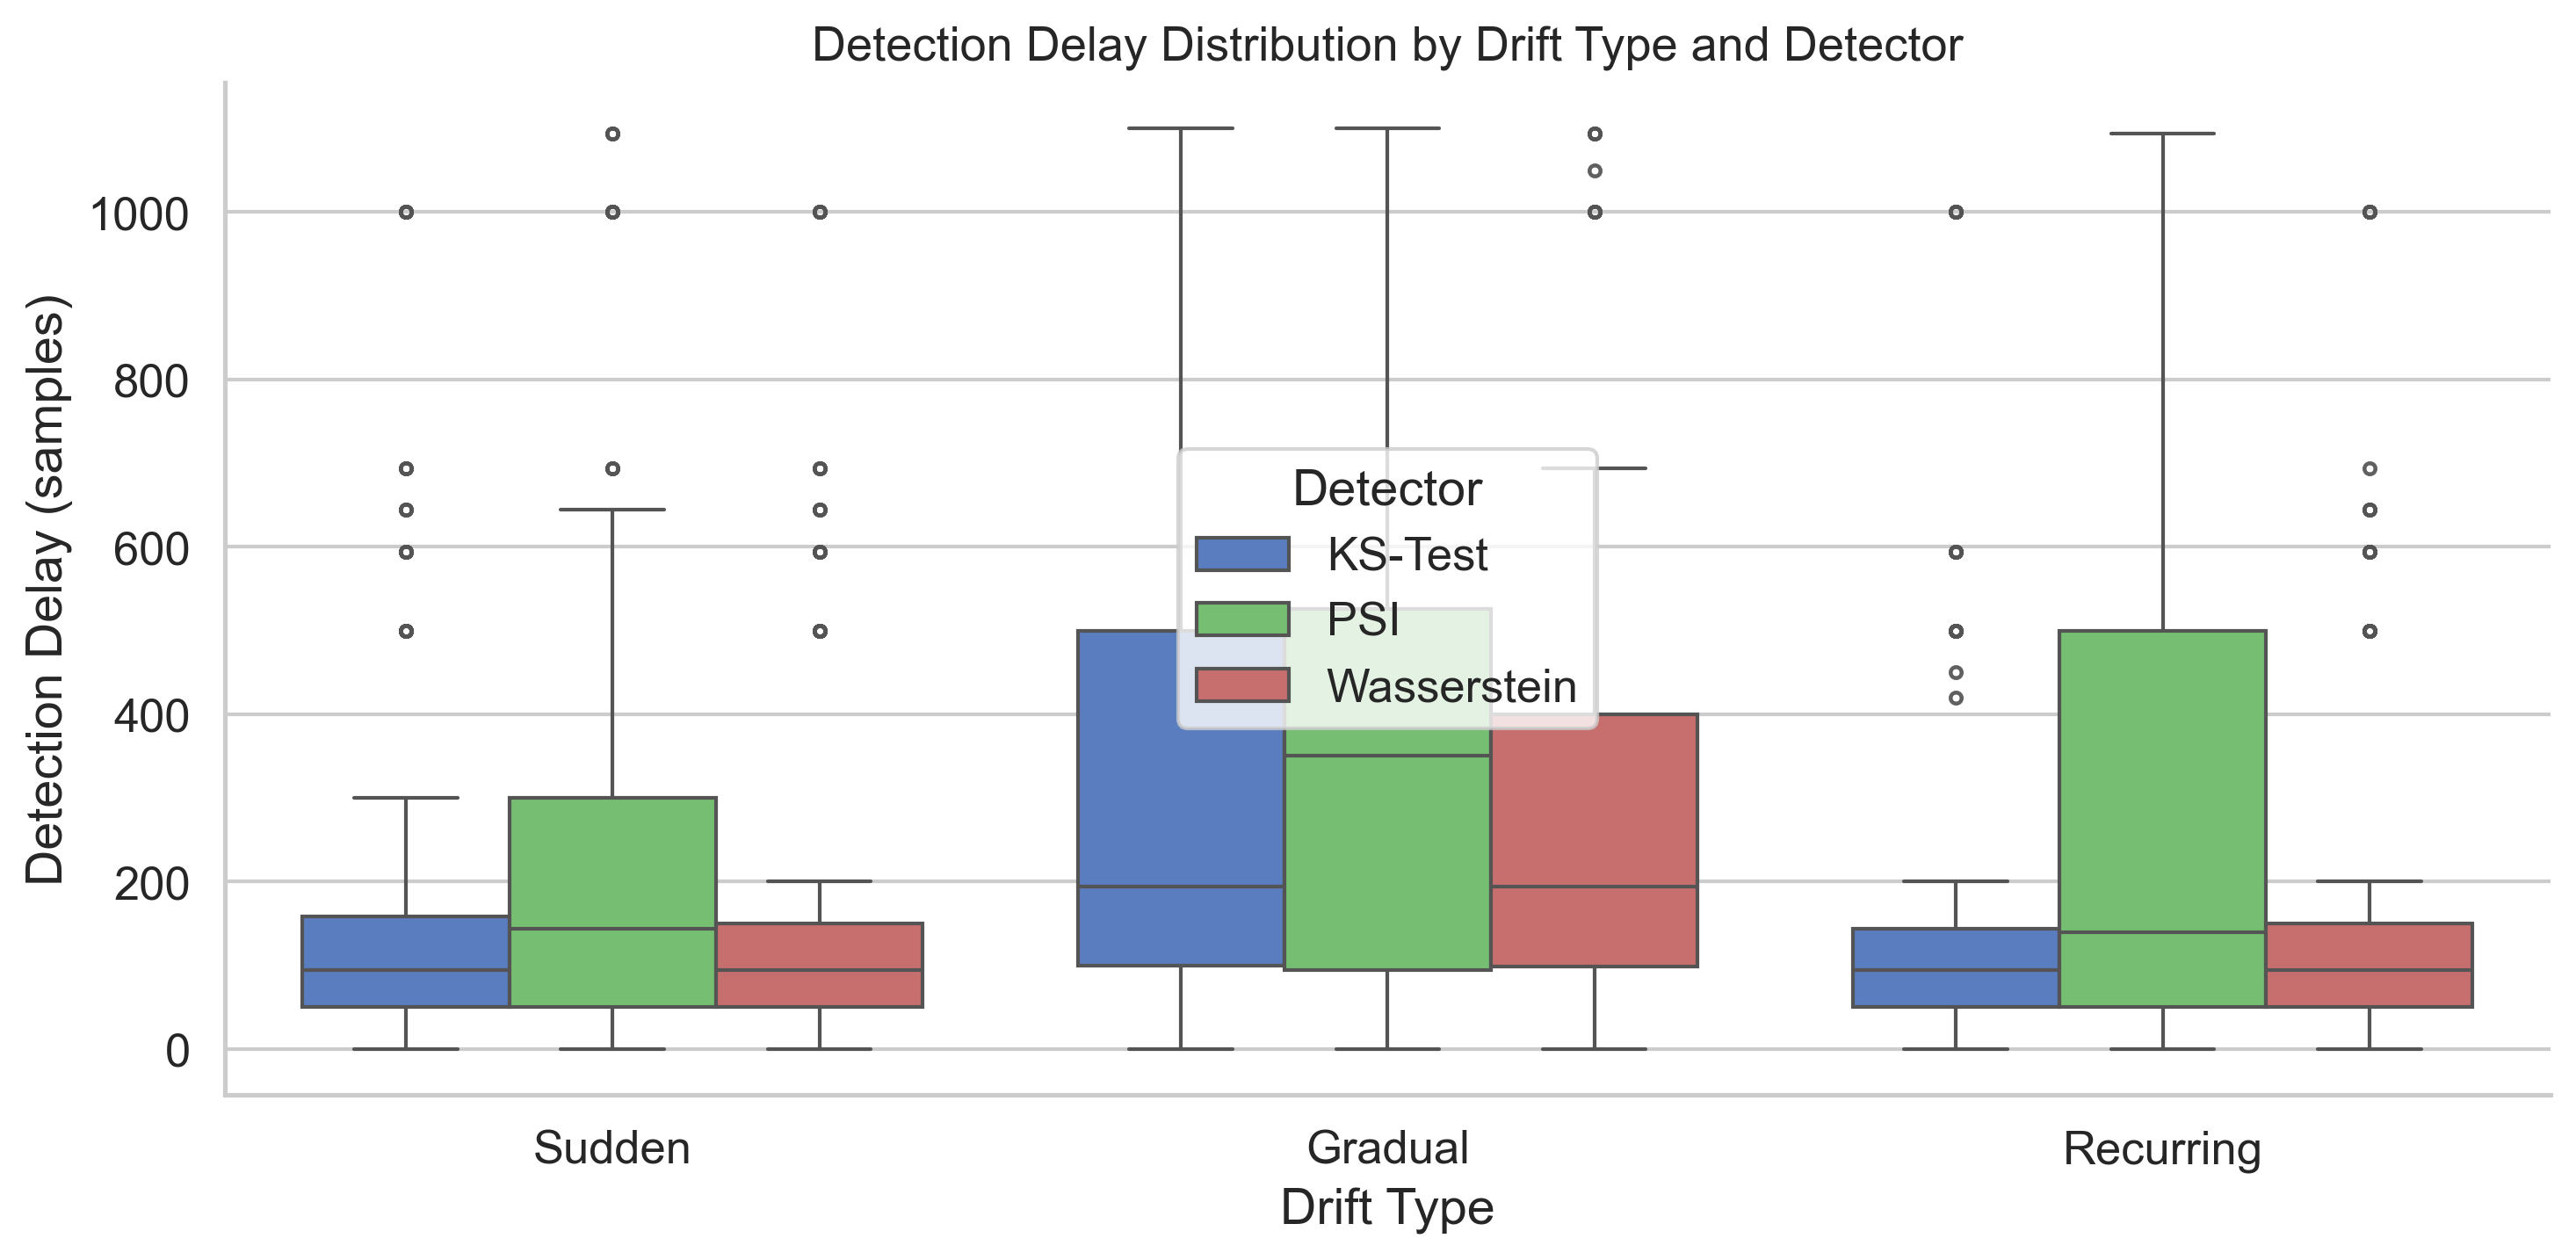
\includegraphics[width=0.55\textwidth]{../../04_results/plots/fig6_delay_by_drift_type.png}
\end{center}
\end{frame}

\begin{frame}{RQ3: Constraint Configuration Dominates}
\begin{center}
\Large \textbf{37-fold range} in detection delay\\
\small (22.0 windows best case $\to$ 827.6 windows worst case)
\end{center}
\begin{itemize}
  \item Window size: $\rho = 0.543$ (strongest single effect)
  \item Monitoring frequency: $\rho = 0.487$
  \item Reference size: a \textbf{threshold}, not a scale (500 samples $\approx$ unlimited)
\end{itemize}
\begin{center}
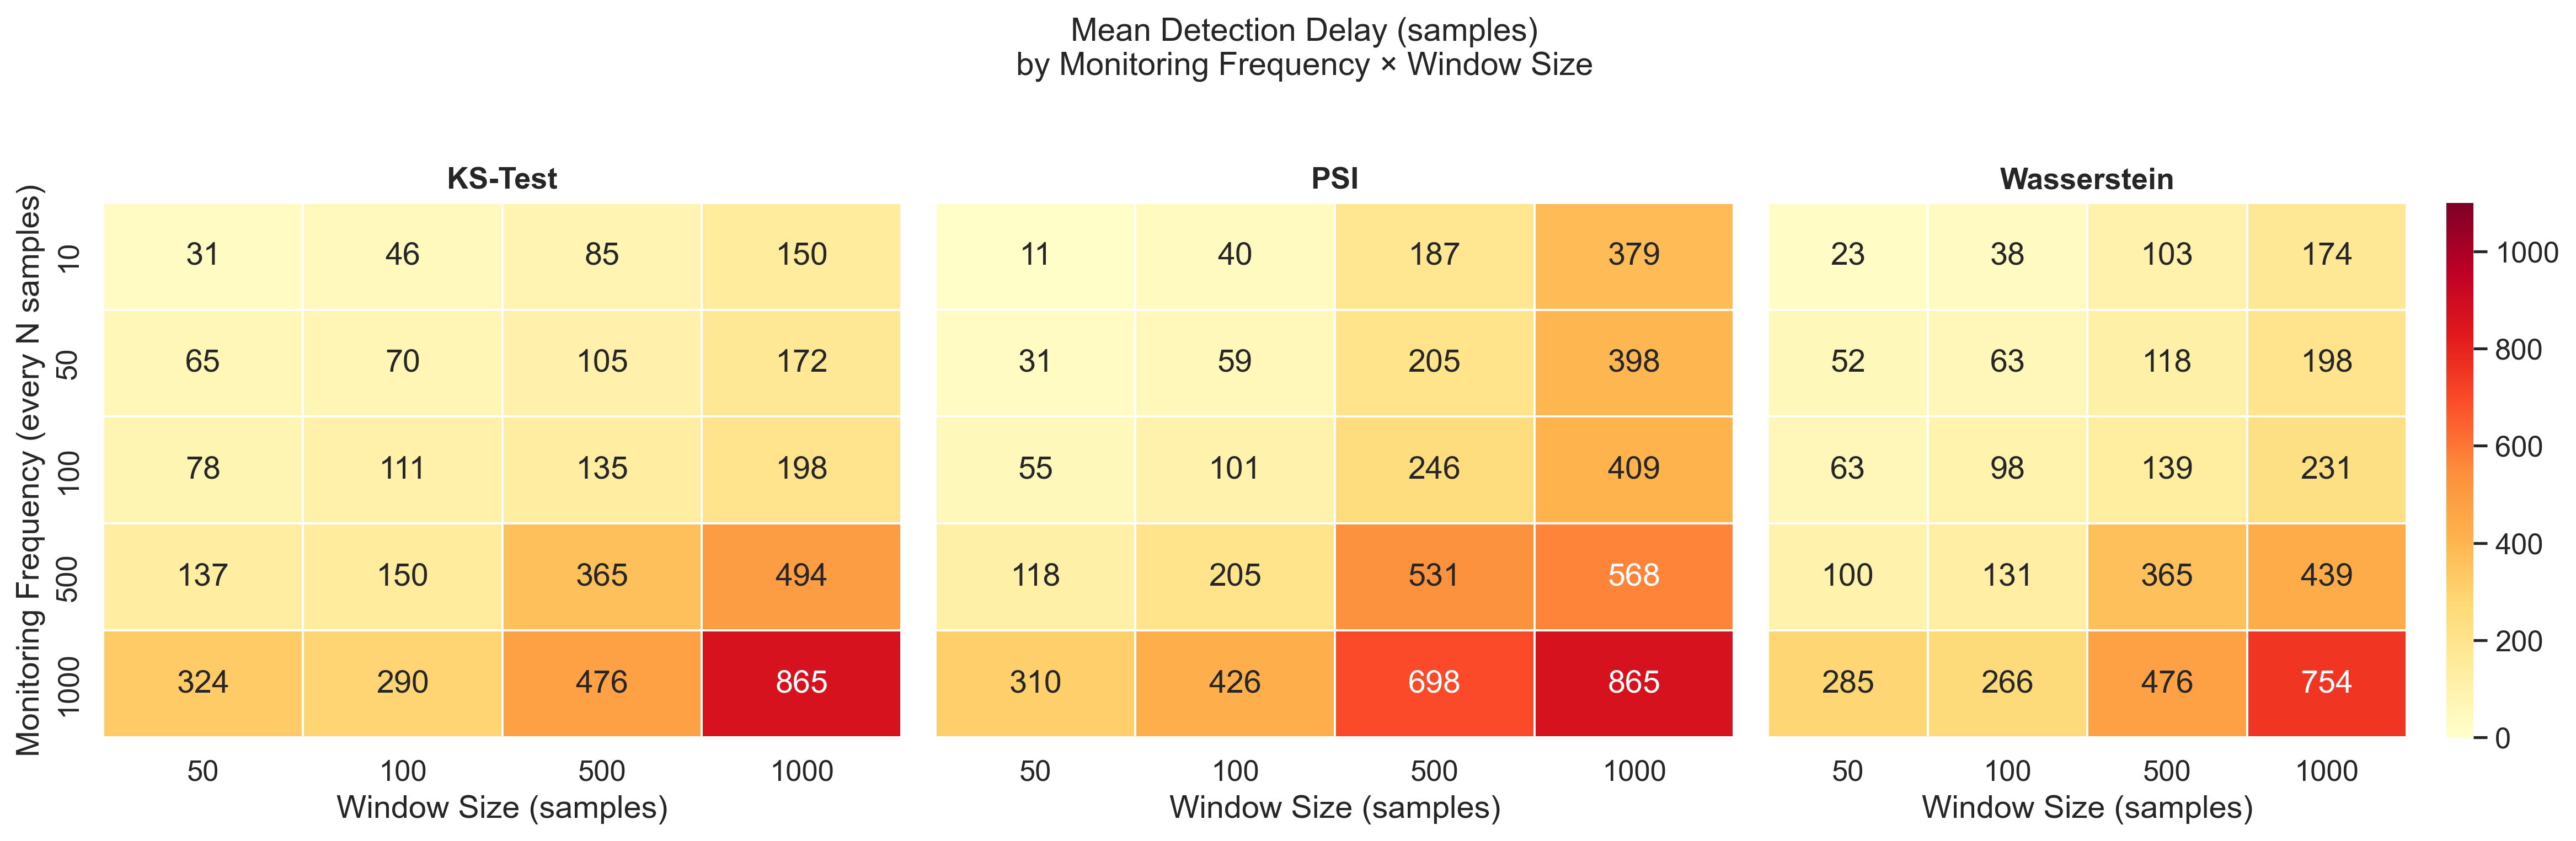
\includegraphics[width=0.68\textwidth]{../../04_results/plots/fig1_delay_heatmap.png}
\end{center}
\end{frame}

\begin{frame}{RQ4: Model Robustness Under Drift}
\begin{itemize}
  \item \textbf{Random Forest} degrades least under drift
  \item vs.\ LightGBM: $r=-0.383$ (medium) \quad vs.\ Log.\ Reg.: $r=-0.185$ (small)
  \item Mechanism: bagging + feature-subset randomisation \textbf{decorrelates} trees, so a shift in one feature does not propagate to the whole ensemble
  \item LightGBM's sequential boosting \textbf{propagates} shift-induced error across rounds
\end{itemize}
\begin{center}
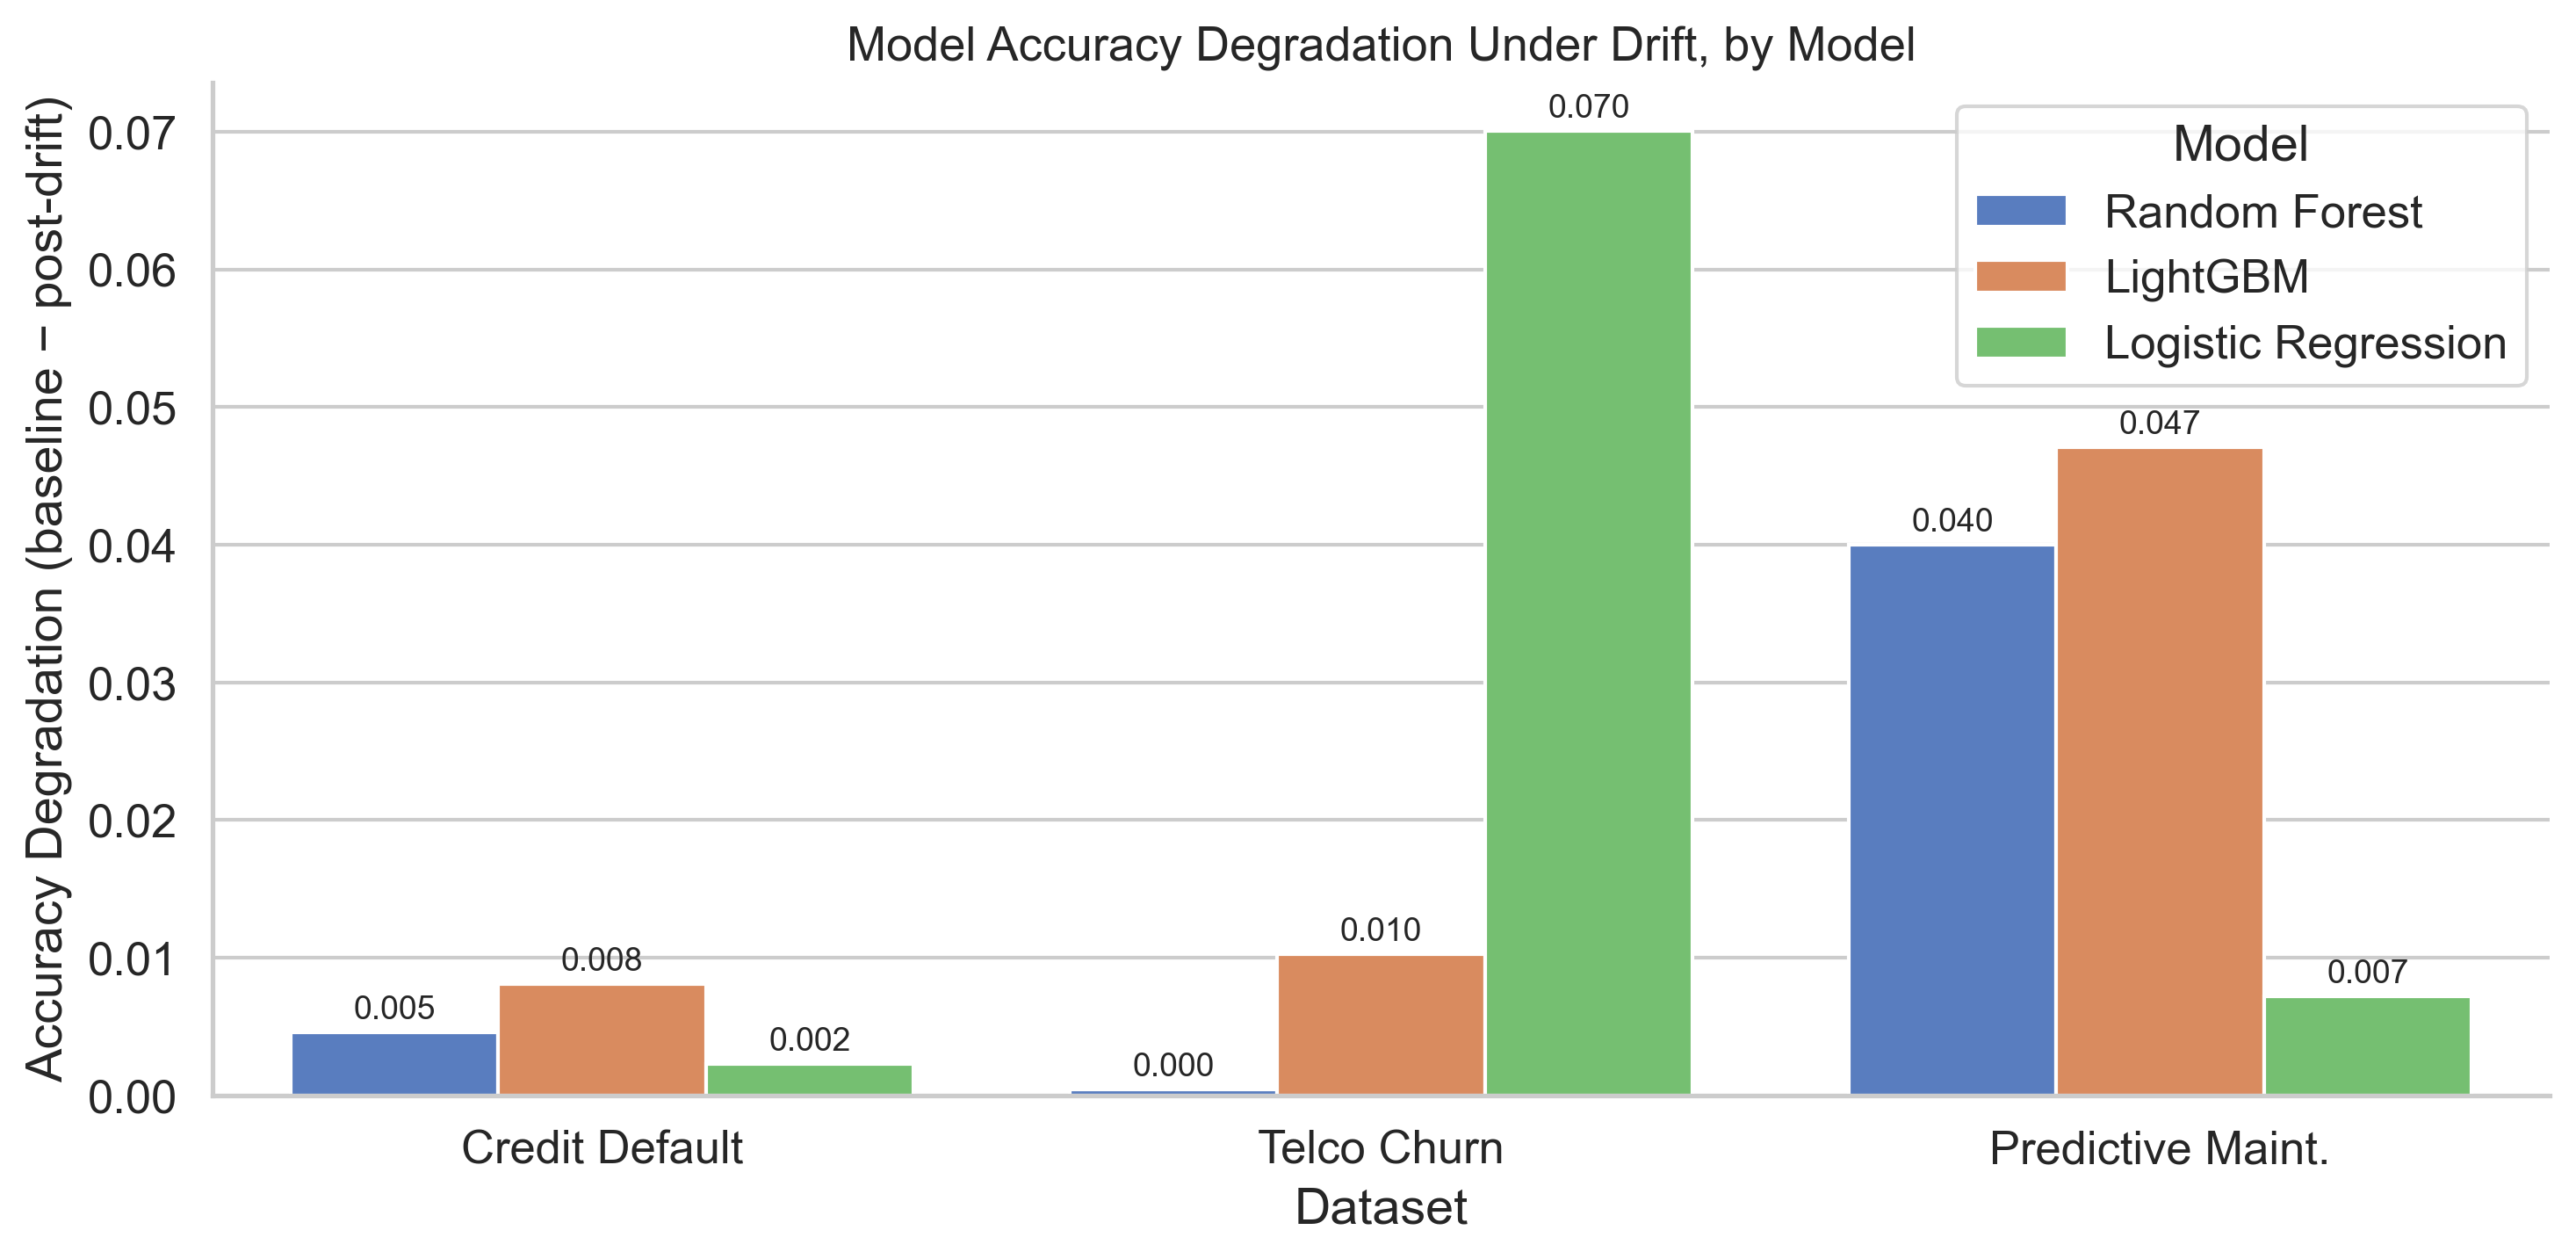
\includegraphics[width=0.68\textwidth]{../../04_results/plots/fig8_model_robustness.png}
\end{center}
\end{frame}

\begin{frame}{Priority Hierarchy for Practitioners}
\begin{enumerate}
  \item \textbf{Monitoring regime first}: frequency \& window size (37$\times$ impact)
  \item \textbf{Drift type awareness second}: gradual drift needs tighter configuration
  \item \textbf{Detector/model choice third}: secondary; choose on cost or robustness, not raw performance
\end{enumerate}
\vspace{1em}
\begin{block}{Reframing}
The field asks ``which algorithm is best?'' This study shows: \textbf{ask how it is configured first.}
\end{block}
\end{frame}

\begin{frame}{Limitations \& Next Steps}
\textbf{Limitations}
\begin{itemize}
  \item Synthetic/injected drift, not organic real-world drift
  \item Univariate detection only (per-feature, not correlation structure)
  \item 3 datasets, tabular binary classification only
\end{itemize}
\textbf{For discussion}
\begin{itemize}
  \item Testing scale-sensitivity via distribution-preserving synthetic expansion (not duplication)
  \item Candidate venues: IEEE COMPSAC SRS, SAICSIT 2026
  \item Chapter 5/6 merge decision
\end{itemize}
\end{frame}

\end{document}
